\section{Wellen}
\subsection{Wellengeschwindigkeit}

\begin{center}
	\begin{minipage}{0.4\textwidth}
		\unitText{$u_L$}{Elastische Longitudinalwellen}{$\frac{m}{s}$}
	\end{minipage}%%% to prevent a space
	\begin{minipage}{0.2\textwidth}
		\formula{$u_L = \sqrt{\dfrac{E}{\varrho}}$}
	\end{minipage}
\end{center}
\begin{center}
	\begin{minipage}{0.4\textwidth}
		\unitText{$u_T$}{Elastische Transversalwellen}{$\frac{m}{s}$}
	\end{minipage}%%% to prevent a space
	\begin{minipage}{0.2\textwidth}
		\formula{$u_T = \sqrt{\dfrac{G}{\varrho}}$}
	\end{minipage}
\end{center}
\begin{center}
	\begin{minipage}{0.4\textwidth}
		\unitText{$u_T$}{Transversalwellen auf einem Seil oder einer Saite}{$\frac{m}{s}$}
	\end{minipage}%%% to prevent a space
	\begin{minipage}{0.2\textwidth}
		\formula{$u_T = \sqrt{\dfrac{F}{\varrho A}}$}
	\end{minipage}
\end{center}
\begin{center}
	\begin{minipage}{0.4\textwidth}
		\unitText{$u_S$}{Schwerewellen in tiefem Wasser}{$\frac{m}{s}$}
	\end{minipage}%%% to prevent a space
	\begin{minipage}{0.2\textwidth}
		\formula{$u_S = \sqrt{\dfrac{g \lambda}{2 \pi}}$}
	\end{minipage}
\end{center}
\begin{center}
	\begin{minipage}{0.4\textwidth}
		\unitText{$u_S$}{Schwerewellen in flachem Wasser}{$\frac{m}{s}$}
	\end{minipage}%%% to prevent a space
	\begin{minipage}{0.2\textwidth}
		\formula{$u_S = \sqrt{g h}$}
	\end{minipage}
\end{center}
\begin{center}
	\begin{minipage}{0.4\textwidth}
		\unitText{$u_K$}{Kapillarwellen}{$\frac{m}{s}$}
	\end{minipage}%%% to prevent a space
	\begin{minipage}{0.2\textwidth}
		\formula{$u_K = \sqrt{\dfrac{2 \pi \sigma}{\varrho \lambda}}$}
	\end{minipage}
\end{center}
\begin{center}
	\begin{minipage}{0.3\textwidth}
		\unitText{$u$}{Schallwellen in Fluiden}{$\frac{m}{s}$}
	\end{minipage}%%% to prevent a space
	\begin{minipage}{0.3\textwidth}
		\formula{$u = \sqrt{\dfrac{1}{\varrho \kappa}}$}
	\end{minipage}
\end{center}
\begin{center}
	\begin{minipage}{0.3\textwidth}
		\unitText{$u_G$}{Schallwellen in Gasen}{$\frac{m}{s}$}
	\end{minipage}%%% to prevent a space
	\begin{minipage}{0.3\textwidth}
		\formula{$u_G = \sqrt{\dfrac{\varkappa p}{\varrho}}$}
		\formula{$u_G = \sqrt{\dfrac{\varkappa R T}{M}}$}
	\end{minipage}
\end{center}
\begin{center}
	\begin{minipage}{0.3\textwidth}
		\unitText{$u_G$}{elektromagnetische Wellen}{$\frac{m}{s}$}
	\end{minipage}%%% to prevent a space
	\begin{minipage}{0.3\textwidth}
		\formula{$u = \dfrac{c}{n}$}
	\end{minipage}
\end{center}

\begin{center}
	\begin{minipage}{0.3\textwidth}
		\unitText{$A$}{Fläche}{$m^2$} \\
		\unitText{$E$}{Elastizitätsmodul}{$\frac{N}{m^2}$} \\
		\unitText{$F$}{Spannkraft}{$N$} \\
		\unitText{$G$}{Schubmodul}{$\frac{N}{m^2}$} \\
		\unitText{$M$}{Molmasse}{$\frac{kg}{mol}$} \\
		\unitText{$R$}{Universale Gas-Konstante (8.3145)}{$\frac{J}{K mol}$} \\
		\unitText{$T$}{absolute Temperatur}{$K$} \\
		\unitText{$c$}{Lichtgeschwindigkeit}{$\frac{m}{s}$} \\
		\unitText{$g$}{Erdbeschleunigung}{$\frac{m}{m^s}$}
	\end{minipage}%%% to prevent a space
	\begin{minipage}{0.3\textwidth}
		\unitText{$h$}{Wassertiefe}{$m$} \\
		\unitText{$n$}{Brechungsindex}{$1$} \\
		\unitText{$p$}{Druck}{$Pa$} \\
		\unitText{$u$}{Wellengeschwindigkeit}{$\frac{m}{s}$} \\
		\unitText{$\kappa$}{Kompressibilität}{$Pa$} \\
		\unitText{$\varkappa$}{Adiabatenexponent}{$1$} \\
		\unitText{$\lambda$}{Wellenlänge}{$m$} \\
		\unitText{$\varrho$}{Dichte}{$\frac{kg}{m^3}$} \\
		\unitText{$\sigma$}{Oberflächenspannung}{$\frac{N}{m}$}
	\end{minipage}
\end{center}

\begin{center}
	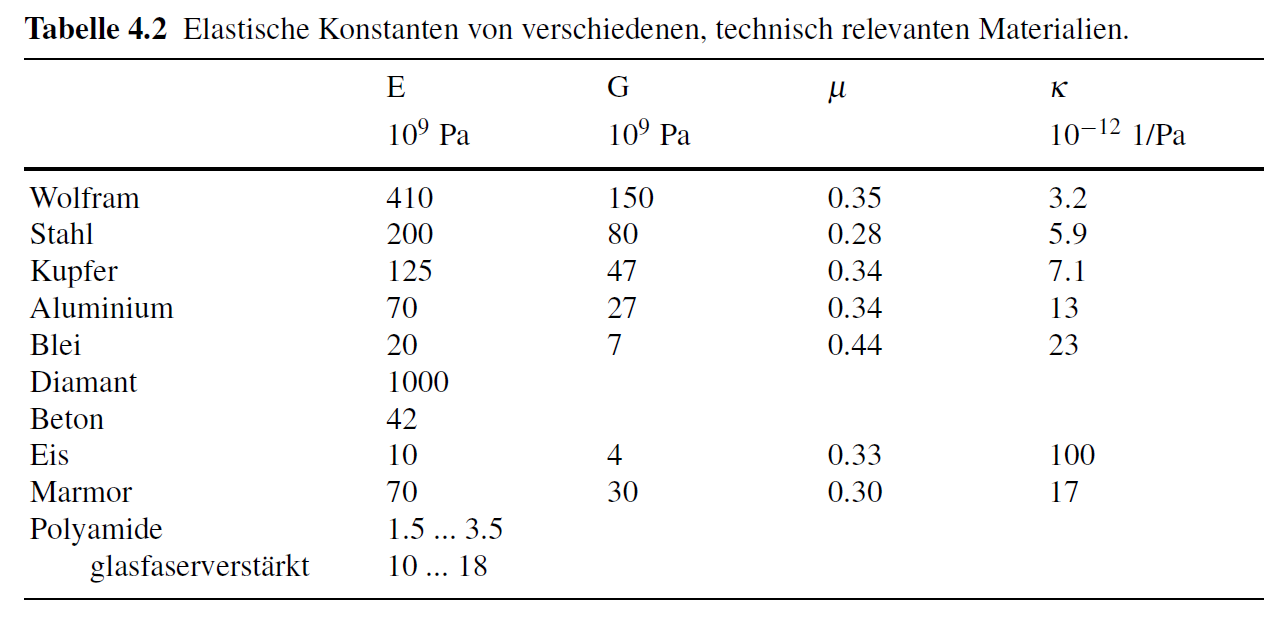
\includegraphics[height=5.5cm,keepaspectratio=true]{Images/elastische_konstanten.png}
\end{center}


\subsection{Harmonische Wellen}
\begin{center}
	\begin{minipage}{0.2\textwidth}
		\formula{$u = \dfrac{\omega}{k}$}
		\formula{$\lambda = \dfrac{2 \pi}{k} = \dfrac{u}{f}$}
		\formula{$k = \dfrac{2 \pi}{\lambda}$}
		\formula{$\omega = \dfrac{2 \pi}{T}$}
		\formula{$f = \dfrac{1}{T}$}
		
	\end{minipage}%%% to prevent a space
	\begin{minipage}{0.3\textwidth}
		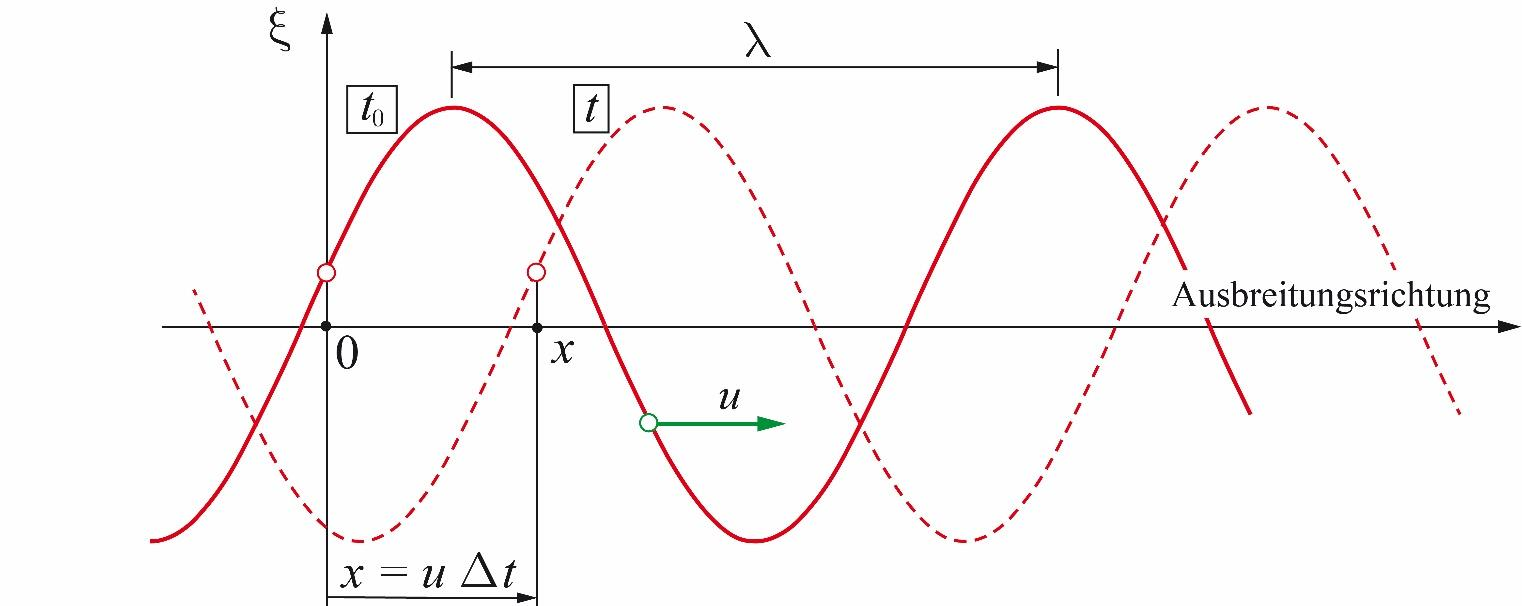
\includegraphics[height=3cm,keepaspectratio=true]{Images/harmonische_welle.png}
	\end{minipage}
\end{center}




\subsection{Wellenausbreitung}
\subsubsection{Akustischer Doppler Effekt}
\formula{$u = \sqrt{\dfrac{\varkappa R T}{M}}$}
\begin{center}
	\begin{minipage}{0.3\textwidth}
		\textbf{Bewegte Quelle:}\\
		\formula{$f' = \dfrac{1}{1 \mp \dfrac{v_Q}{u}} f$}
		\formula{$f' = \dfrac{u}{\lambda'}$}
		\formula{$\lambda' = \lambda - v_Q t$}
	\end{minipage}%%% to prevent a space
	\begin{minipage}{0.2\textwidth}
		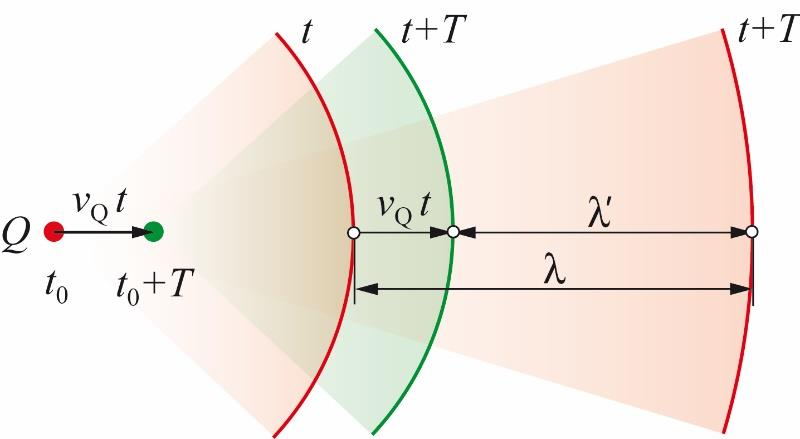
\includegraphics[height=3cm,keepaspectratio=true]{Images/akustischer_doppler_effekt_bewegte_quelle.png}
	\end{minipage}
\end{center}
\begin{center}
	\begin{minipage}{0.2\textwidth}
		\textbf{Bewegter Quelle, unter Winkel:}\\
		\formula{$f' = \dfrac{1}{1 - \dfrac{v_Q}{u} \cos(\vartheta_Q)}$}
	\end{minipage}%%% to prevent a space
	\begin{minipage}{0.3\textwidth}
		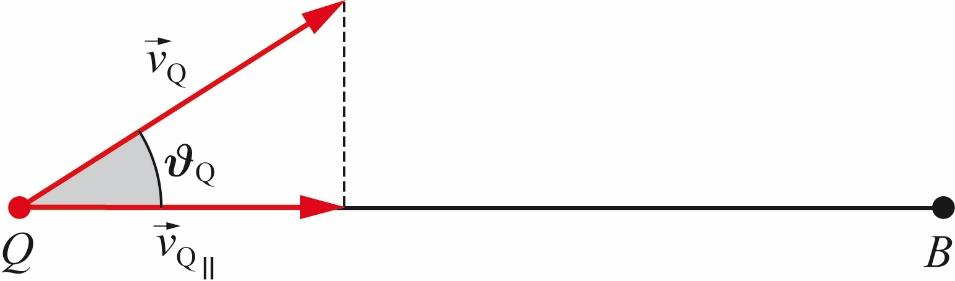
\includegraphics[height=2cm,right,keepaspectratio=true]{Images/akustischer_doppler_effekt_bewegte_quelle_unter_winkel.png}
	\end{minipage}
\end{center}
\begin{center}
	\begin{minipage}{0.2\textwidth}
		\textbf{Bewegter Beobachter:}\\
		\formula{$f' = (1 \pm \dfrac{v_B}{u}) f$}
	\end{minipage}%%% to prevent a space
	\begin{minipage}{0.3\textwidth}
		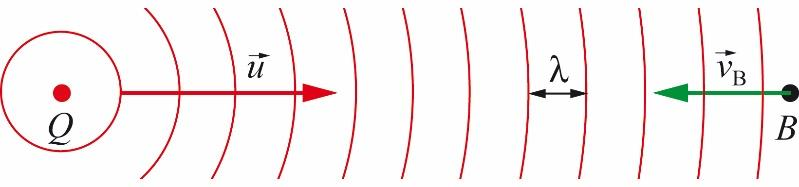
\includegraphics[height=1.5cm,right,keepaspectratio=true]{Images/akustischer_doppler_effekt_bewegter_beobachter.png}
	\end{minipage}
\end{center}
\begin{center}
	\begin{minipage}{0.3\textwidth}
		\textbf{Bewegter Beobachter und bewegte Quelle:}\\
		\formula{$f_B = \dfrac{u + v_B \cos(\vartheta_B)}{u - v_Q \cos(\vartheta_Q)} f_Q$}
	\end{minipage}%%% to prevent a space
	\begin{minipage}{0.2\textwidth}
		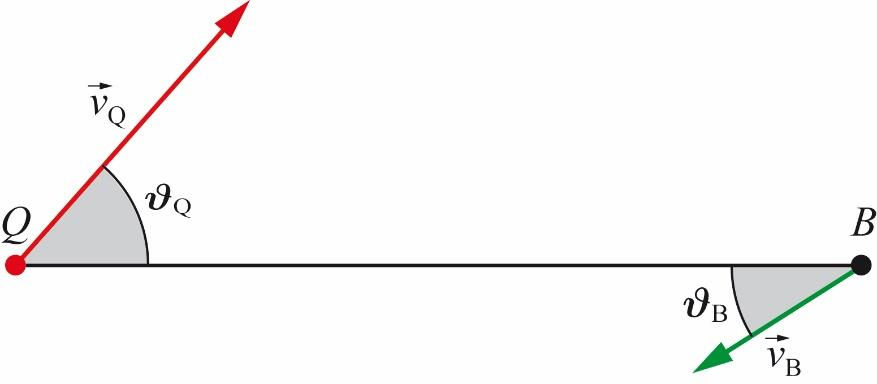
\includegraphics[height=2cm,right,keepaspectratio=true]{Images/akustischer_doppler_effekt_bewegter_beobachter_bewegte_quelle.png}
	\end{minipage}
\end{center}

\begin{minipage}{0.25\textwidth}
	\unitText{$u$}{Schallgeschwindigkeit}{$\frac{m}{s}$} \\
	\unitText{$f'$}{Frequenz beim Beobachter}{$Hz$} \\
	\unitText{$v_Q$}{Geschwindigkeit der Quelle}{$\frac{m}{s}$} \\
	\unitText{$v_B$}{Geschwindigkeit des Beobachters}{$\frac{m}{s}$}
\end{minipage}%%% to prevent a space
\begin{minipage}{0.25\textwidth}
	\unitText{$\vartheta_Q$}{Winkel der Quelle}{$rad$} \\
	\unitText{$\vartheta_B$}{Winkel des Beobachters}{$rad$} \\
	\unitText{$\varkappa$}{Adiabatenexponent}{$1$} \\
	\unitText{$\lambda$}{Wellenlänge}{$m$}
\end{minipage}






\subsubsection{Optischer Doppler Effekt}
\formula{$f' = \dfrac{\sqrt{1 - \beta^2}}{1 - \beta \cos(\vartheta)} f$}
\formula{$\beta = \dfrac{v}{c}$}

\unitText{$v$}{Geschwindigkeit (Quelle oder Betrachter, eggal)}{$\frac{m}{s}$}\\
\unitText{$c$}{Lichtgeschwindigkeit}{$\frac{m}{s}$}




\subsubsection{Machkegel}
\begin{center}
	\begin{minipage}{0.1\textwidth}
		\formula{$\sin(\vartheta) = \dfrac{u}{v}$}
	\end{minipage}%%% to prevent a space
	\begin{minipage}{0.4\textwidth}
		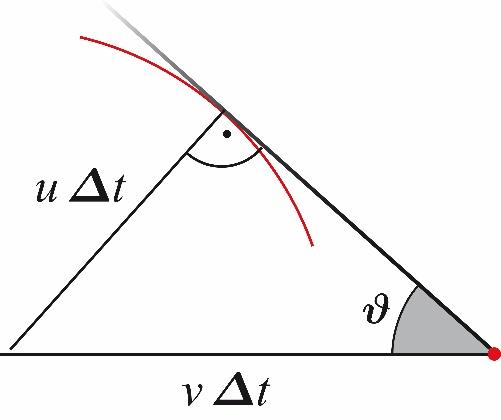
\includegraphics[height=3cm,keepaspectratio=true]{Images/machkegel.png}
		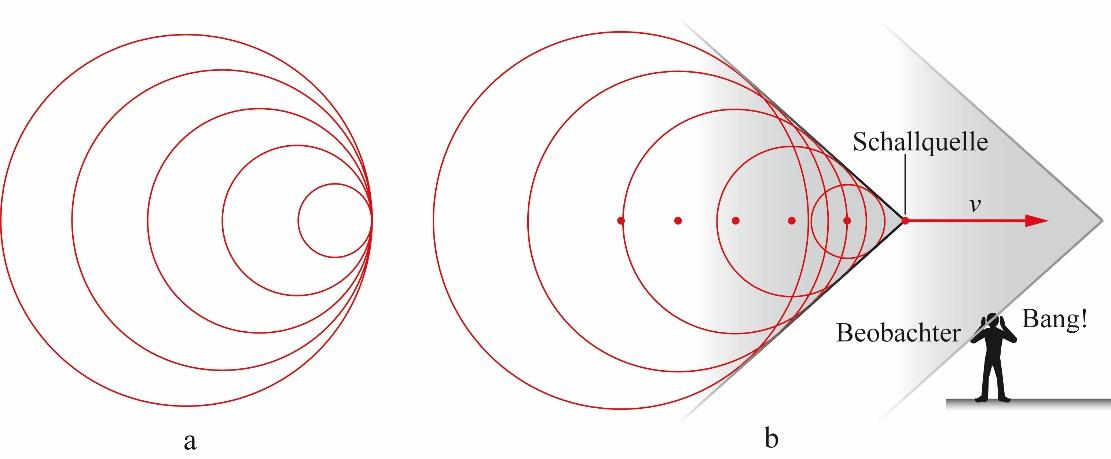
\includegraphics[height=3cm,keepaspectratio=true]{Images/machkegel_vorher_nachher.png}
	\end{minipage}
\end{center}


\subsubsection{Schwebung}
\begin{center}
	\begin{minipage}{0.2\textwidth}
		\formula{$f_s = f_1 - f_2$}
	\end{minipage}%%% to prevent a space
	\begin{minipage}{0.3\textwidth}
		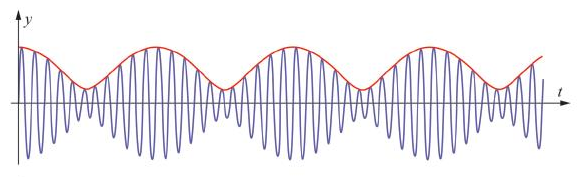
\includegraphics[height=2cm,keepaspectratio=true]{Images/schwebung.png}
	\end{minipage}
\end{center}




\subsection{Wellenwiderstand, Energietransport}
\subsubsection{Schallwellen}
\begin{center}
	\begin{minipage}{0.2\textwidth}
		\formula{$\tilde{p}(x,t) = \Delta p_0 \cos(\omega t - k x)$}
		\formula{$\Delta p_0 = \varrho u \omega \xi_0 =\rho u v_0$}
		\formula{$v = v_0 \cos(\omega t - k x)$}
		\formula{$v_0 = \omega \xi_0$}
		\formula{$Z = \varrho u$}
		\formula{$\Delta p_0 = Z \cdot v_0$}
		\formula{$I = \frac{1}{2} \varrho v^2_0 u$}
	\end{minipage}%%% to prevent a space
	\begin{minipage}{0.3\textwidth}
		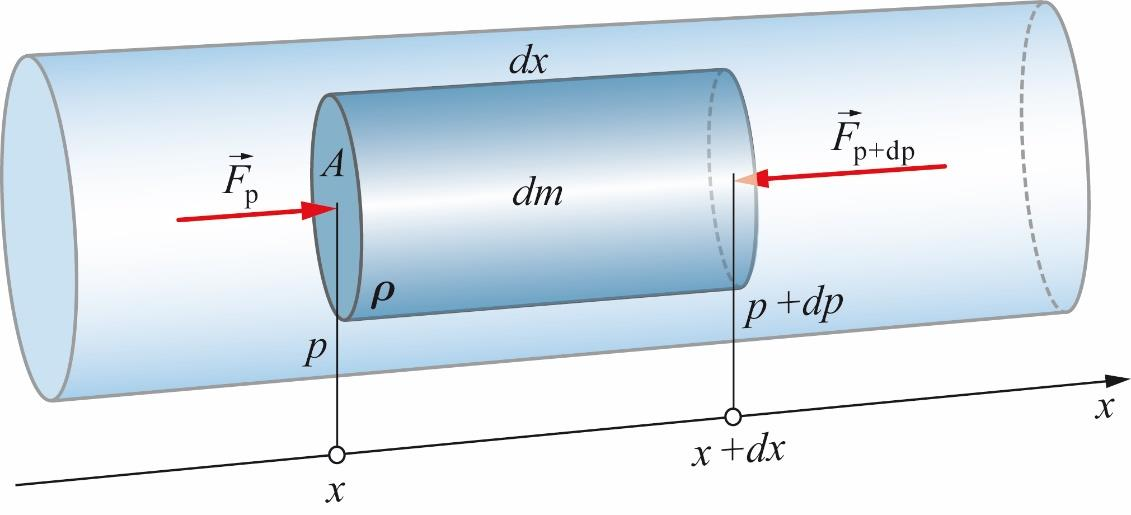
\includegraphics[height=3cm,right,keepaspectratio=true]{Images/schallwellen_kinematik_newton.png}
	\end{minipage}
\end{center}

\unitText{$\tilde{p}$}{Schalldruck}{$Pa$}\\
\unitText{$\Delta p_0$}{Schalldruck mit Amplitude}{$Pa$}\\
\unitText{$\varrho$}{Druck}{$Pa$}
\unitText{$v$}{Schallschnelle}{$\frac{m}{s}$}\\
\unitText{$v_0$}{Schallschnelle mit Schnelleamplitude}{$\frac{m}{s}$}\\
\unitText{$Z$}{Schallwellenimpedanz}{$?$}\\
\unitText{$\Delta p_0$}{Schallwellenimpedanz mit Beziehung}{$?$}\\
\unitText{$I$}{Schallintensität}{$\frac{W}{m^2}$}\\
\unitText{$\xi_0$}{Maximale Auslenkung}{$...$}





\subsection{Dispersion}
\subsubsection{Saitenschwingung}
\formula{$u = \sqrt{\dfrac{F}{\varrho A}}$}
\subsubsection{Balken}
\formula{$u(\lambda) = \dfrac{\omega}{k} = 
	\sqrt{\left( \dfrac{F}{\varrho A} + \dfrac{\pi E A}{\varrho \lambda^2} \right) }$}
\subsubsection{Wasserwellen}


\begin{center}
	\begin{minipage}{0.3\textwidth}
		\formula{$u(\lambda) = \sqrt{\left( \dfrac{g \lambda}{2 \pi} + \dfrac{2 \pi \sigma}{\varrho \lambda} \right) \tanh \left( \dfrac{2 \pi h}{\lambda} \right) }$}
	\end{minipage}%%% to prevent a space
	\begin{minipage}{0.2\textwidth}
		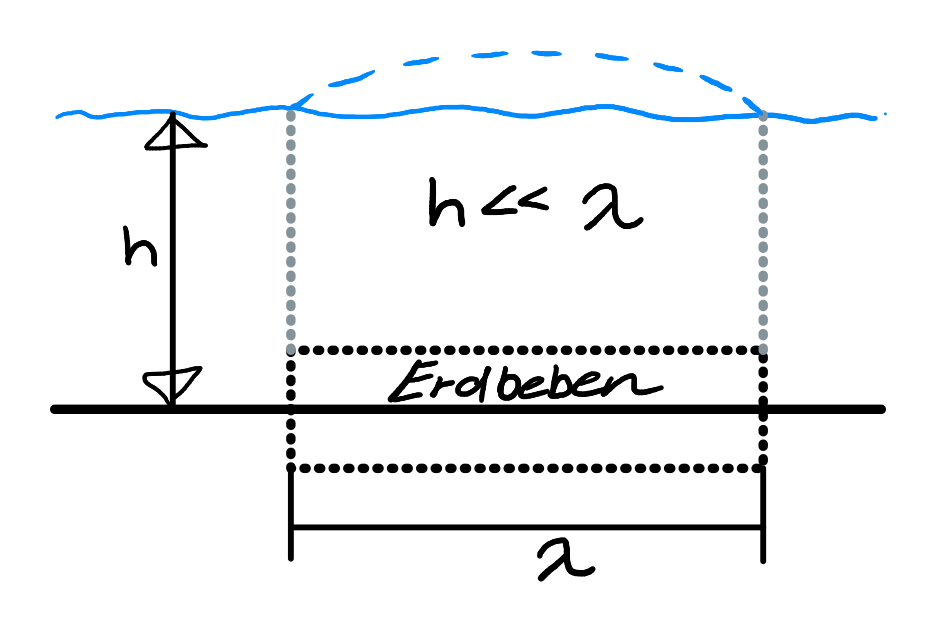
\includegraphics[height=3cm,keepaspectratio=true]{Images/Wasserwelle.png}
	\end{minipage}
\end{center}


\subsection{Überlagerung von Wellen}
\begin{center}
	\begin{minipage}{0.3\textwidth}
		\formula{$\xi_{oben}(x_p, t) = A \sin(\omega t - k \cdot s_A + \varphi_1)$}
		\formula{$\xi_{unten}(x_p, t) = A \sin(\omega t - k \cdot s_B + \varphi_2)$}
		\formula{$\xi_{total} = 2 A \cos \left(k \dfrac{s_B - s_A}{2} \right) \sin \left(\omega t - k \dfrac{s_A + s_B}{2} \right)$}
		\formula{$\Delta s = n \cdot \lambda \Rightarrow \text{Amplitude maximal}$}
	\end{minipage}%%% to prevent a space
	\begin{minipage}{0.2\textwidth}
		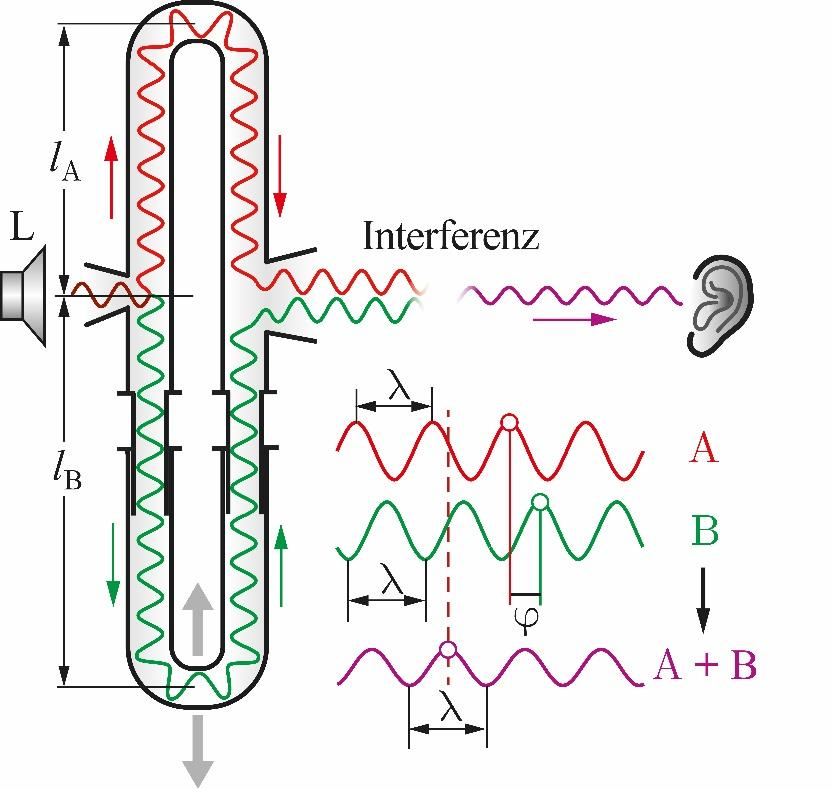
\includegraphics[height=4.5cm,right,keepaspectratio=true]{Images/wellen_ueberlagerung_selbe_quelle.png}
	\end{minipage}
\end{center}

\unitText{$A$}{Maximale Amplitude}{$...$}\\
\unitText{$t$}{Zeit}{$s$}
\unitText{$s_{A}$}{Obere Strecke}{$m$}\\
\unitText{$s_{B}$}{untere Strecke}{$m$}\\
\unitText{$\xi$}{Resultierende Auslenkung}{$...$}\\
\unitText{$\omega$}{Kreisfrequenz}{$\frac{1}{s}$}\\







\subsection{Reflexion und Transmission}
\begin{center}
	\begin{minipage}{0.3\textwidth}
		\formula{$R = \left(  \dfrac{Z_1 - Z_2}{Z_1 + Z_2} \right)^2 $}
		\formula{$T = \dfrac{4 Z_1 Z_2}{(Z_1 + Z_2)^2}$}
		\formula{$\text{Akustisch: } Z = \varrho u$}
		\formula{$\text{Elektromagnetisch: } Z = Z_0 \dfrac{c}{n}$}
	\end{minipage}%%% to prevent a space
	\begin{minipage}{0.2\textwidth}
		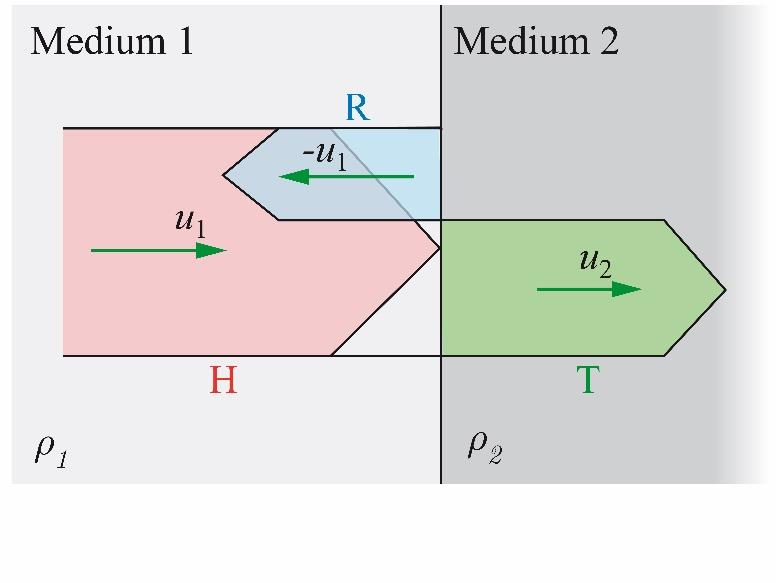
\includegraphics[height=4cm,keepaspectratio=true]{Images/reflexion_und_transmission.png}
	\end{minipage}
\end{center}
\unitText{$R$}{Refflexionskoeffizient}{$?$}\\
\unitText{$T$}{Transmissionskoeffizient}{$?$}\\
\unitText{$Z$}{Impedanz}{$?$}\\
\unitText{$Z_0$}{Vakum-Impedanz (= 377 $\Omega$)}{$?$}\\
\unitText{$\varrho$}{Dichte}{$\frac{kg}{m^3}$}





\subsection{Eigenschwingungen}
\subsubsection{Saite}

\begin{center}
	\begin{minipage}{0.35\textwidth}
		\formula{$\lambda_n = \dfrac{2l}{n}$}
		\formula{$f_n = \dfrac{u}{\lambda_n} = n f_1$}
		\formula{$f_1 = \dfrac{1}{2l} \sqrt{\dfrac{F}{\varrho A}}$}
		\formula{$u = \sqrt{\dfrac{F}{\varrho A}}$}
		\formula{$F = \dfrac{4 l^2}{n^2} \varrho A f^2$}
		\formula{$\Delta f = \left( \dfrac{E_{Sa}(\alpha_{Trag} - \alpha_{Sa})}{8 \varrho_{Sa} l^2 f^2 } -\alpha_{Trag} \right) \Delta T f $}
	\end{minipage}%%% to prevent a space
	\begin{minipage}{0.15\textwidth}
		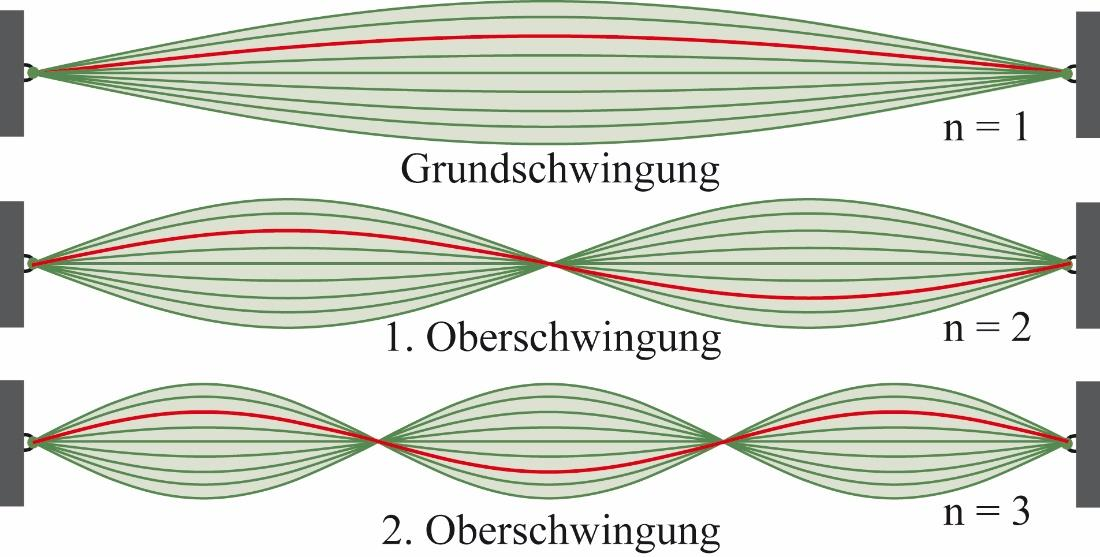
\includegraphics[height=2.5cm,right,keepaspectratio=true]{Images/eigenschwingung_saite.png}
	\end{minipage}
\end{center}
\begin{center}
	\begin{minipage}{0.25\textwidth}
		\unitText{$A$}{Fläche}{$m^2$}\\
		\unitText{$E$}{Elastizitätsmodul}{$\frac{N}{m^2}$}\\
		\unitText{$F$}{Spannkraft}{$N$}\\
		\unitText{$f$}{Frequenz}{$Hz$}\\
		\unitText{$f_1$}{Grundfrequenz}{$Hz$}\\
		\unitText{$l$}{Saitenlänge}{$m$}\\
		\unitText{$n$}{n-te Harmonische}{1}\\
	\end{minipage}%%% to prevent a space
	\begin{minipage}{0.25\textwidth}
		\unitText{$u$}{$Wellengeschwinfigkeit$}{$\frac{m}{s}$}\\
		\unitText{$\lambda$}{Wellenlänge}{$m$}\\
		\unitText{$\varrho$}{Dichte Saite}{$\frac{kg}{m^3}$}\\
		\unitText{$\xi$}{Störung}{$...$}\\
		\unitText{$\omega$}{Kreisfrequenz}{$\frac{1}{s}$}\\
		\unitText{$\alpha$}{Längenausdehnungskoeffizient}{$\frac{1}{K}$}\\
		\unitText{$\varrho$}{Dichte}{$\frac{kg}{m^3}$}
	\end{minipage}
\end{center}




\subsubsection{Pfeife}

\begin{center}
	\begin{minipage}{0.3\textwidth}
		Offene Pfeife:
		\formula{$f_1 = \dfrac{1}{2l} \sqrt{\dfrac{\varkappa R T}{M}} = \dfrac{u}{2l}$}
		\formula{$f_n = n _1$}
		\formula{$\lambda_n = \dfrac{4l}{n} \text{ für } n = 1,3,5,...$}
		\\Gedackte Pfeife:
		\formula{$f_1 = \dfrac{1}{4l} \sqrt{\dfrac{\varkappa R T}{M}} = \dfrac{u}{4l}$}
		\formula{$f_n = n _1$}
		\formula{$\lambda_n = \dfrac{4l}{n} \text{ für } n = 2,4,6,...$}
	\end{minipage}%%% to prevent a space
	\begin{minipage}{0.2\textwidth}
		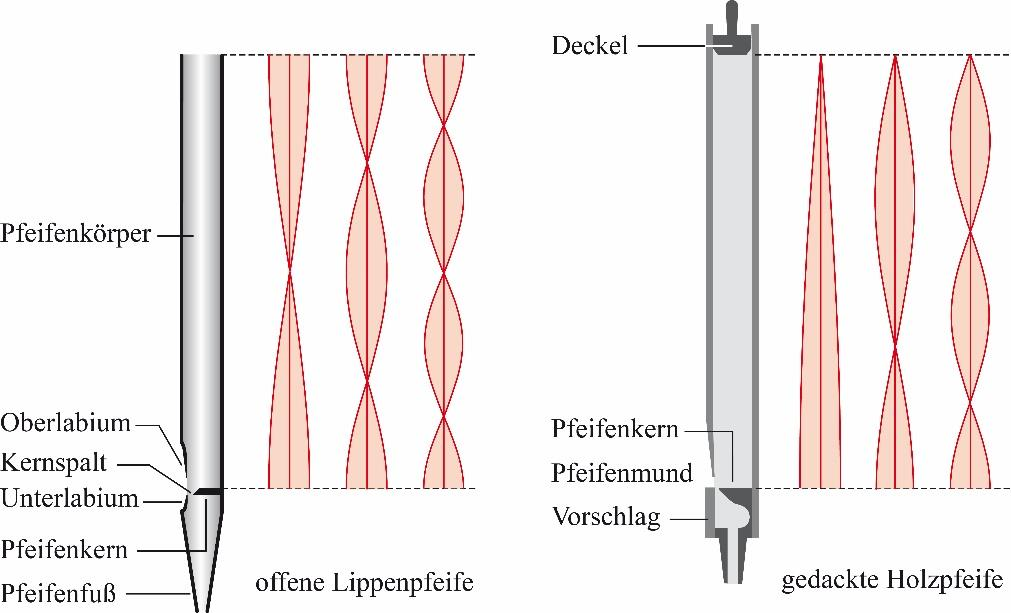
\includegraphics[height=3cm,right,keepaspectratio=true]{Images/eigenschwingung_pfeife.png}
	\end{minipage}
\end{center}
\unitText{$M$}{Molmasse}{$\frac{kg}{mol}$}\\
\unitText{$R$}{universelle Gas-Konstante (=8.3145)}{$\frac{J}{K mol}$}\\
\unitText{$T$}{absolute Temperatur}{$K$}\\
\unitText{$f$}{Frequenz}{$Hz$}\\
\unitText{$f_1$}{Grundfrequenz}{$Hz$}\\
\unitText{$\lambda$}{Wellenlänge}{$m$}\\
\unitText{$\varkappa$}{Adiabatenexponent}{1}\\










\subsubsection{Vorlage}

\begin{center}
	\begin{minipage}{0.3\textwidth}
		
	\end{minipage}%%% to prevent a space
	\begin{minipage}{0.3\textwidth}
		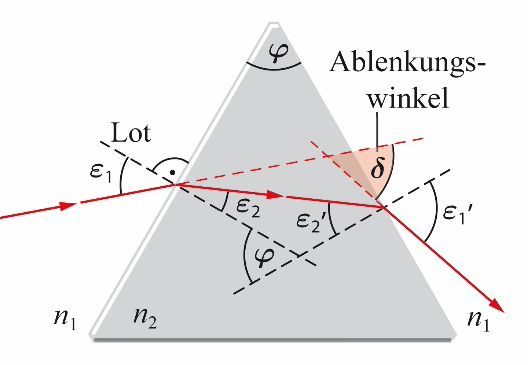
\includegraphics[height=3cm,keepaspectratio=true]{Images/prisma.png}
	\end{minipage}
\end{center}
